% Рисуночки
\section{Конструкторская часть}
\subsection{Описания алгоритмов}

\hspace{1.25cm}
На основании теоретических измышлений были разработаны алгоритмы, реализующие решение задачи коммивояжёра полным перебором и муравьиным алгоритмом. Вариант: ориентированный граф, без элитных муравьёв, карта городов России XVI века. Раз в 60 суток наступает смена летнего сезона на зимний или наоборот. Зимой можно ходить по рекам в обе стороны за равную цену, летом по течению в 2 раза быстрее, против -- в 4 раза медленнее. Незамкнутый маршрут. Блок-схемы этих алгоритмов приведены на рисунках~\ref{fig:block_1} (полный перебор),~\ref{fig:block_1_1} (функция учёта рек и сезона) и~\ref{fig:block_2} (муравьиный алгоритм).

\begin{figure}[H]
    \centering
    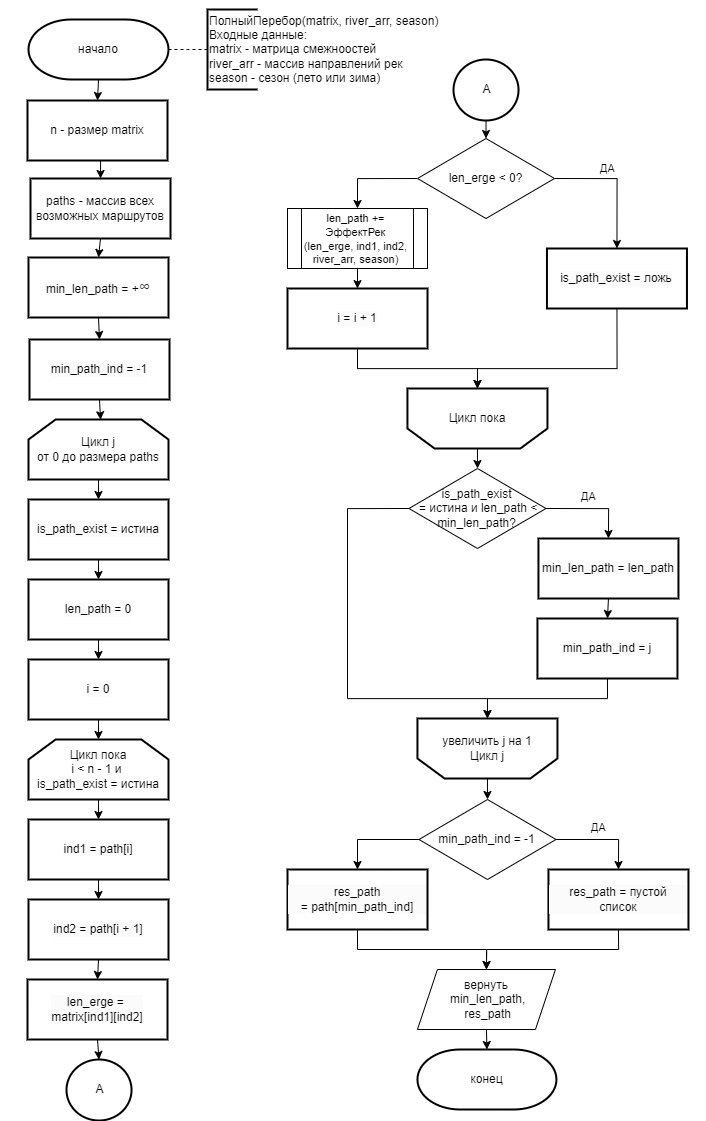
\includegraphics[width=0.9\textwidth]{img/block_full_search.png}
    \caption{Блок-схема алгоритма полного перебора.}
    \label{fig:block_1}
\end{figure}

\begin{figure}[H]
    \centering
    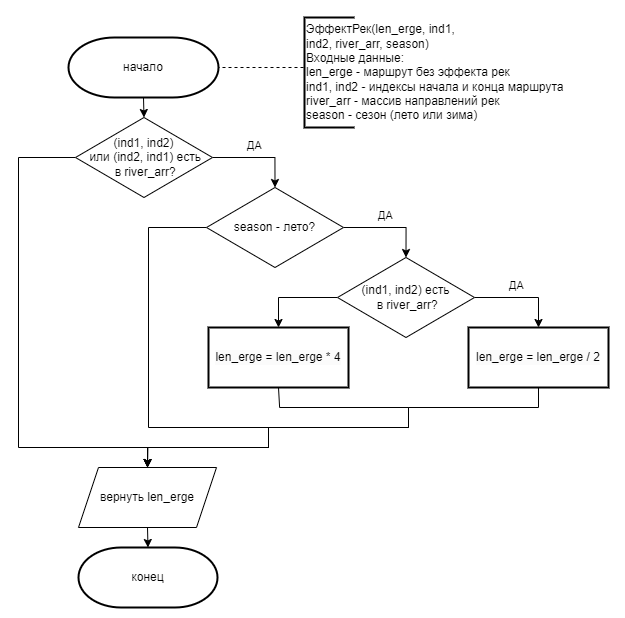
\includegraphics[width=1\textwidth]{img/block_effect_river.png}
    \caption{Блок-схема функции учёта рек и сезона при решении задачи коммивояжёра.}
    \label{fig:block_1_1}
\end{figure}

\begin{figure}[H]
    \centering
    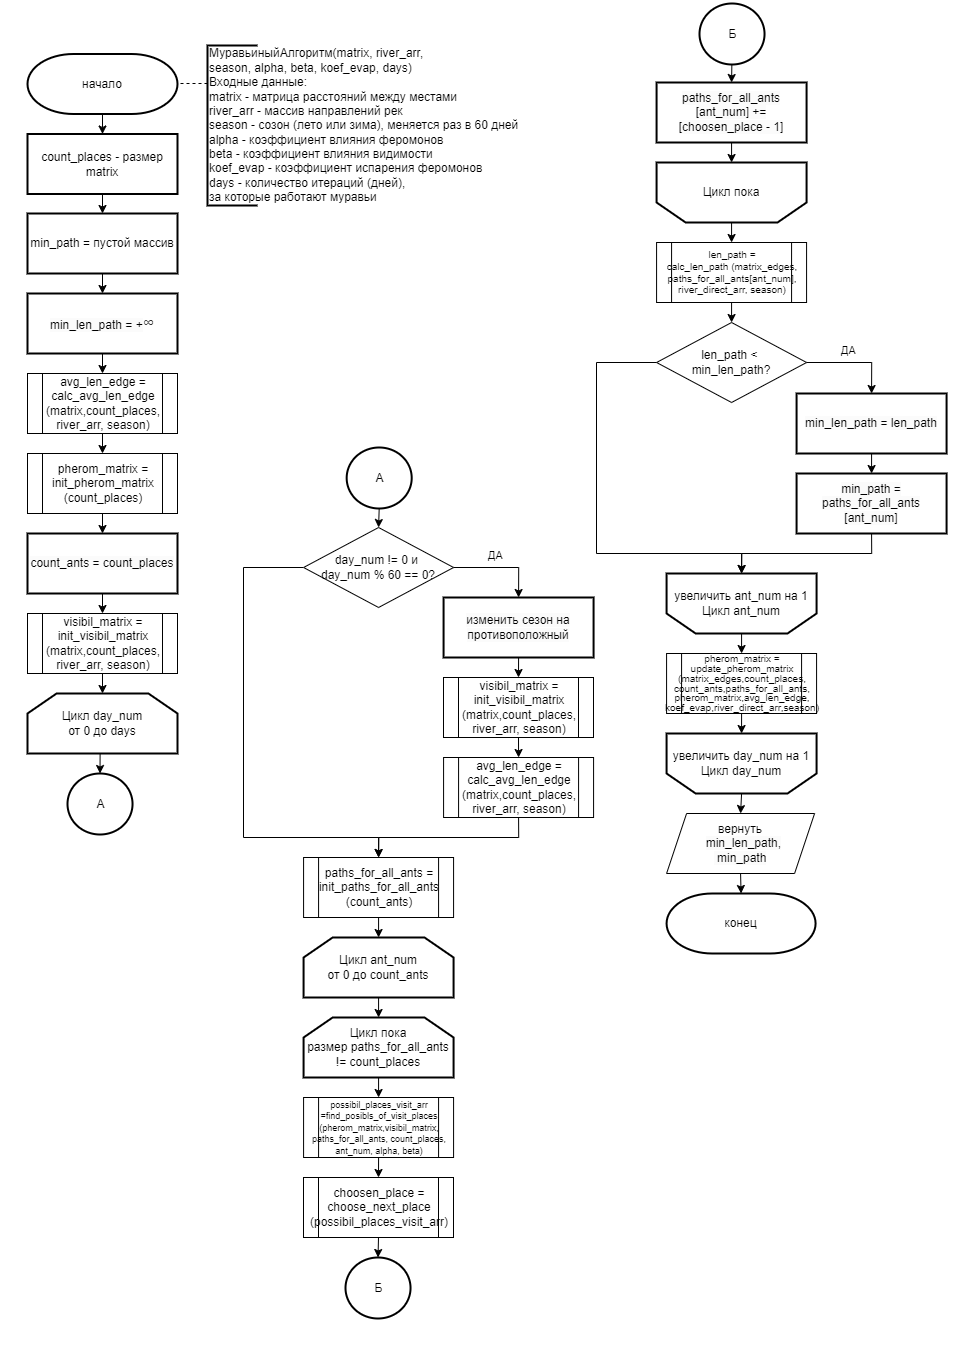
\includegraphics[width=1.1\textwidth]{img/block_ant_algo.png}
    \caption{Блок-схема муравьиного алгоритма.}
    \label{fig:block_2}
\end{figure}

\newpage